% Sample file on how to use subfiles.
\documentclass[ExampleMasters.tex]{subfiles}

\begin{document}
\clearpage


\chapter{Hardware architecture(9 Seiten)}
\label{chap:hardware_setup}

\section{Hardware overview}

\begin{itemize}
	\item give overview of system on truck
	\item sketch for where which unit sits (with numbers to be referenced)
	\item different tasks for Arduino
	\item make communication diagramm with all protocols (CAN, i2c, SPI, serial, ethernet) $<$== this could also be moved to software chapter?
	
\end{itemize}

\begin{figure*}[ph]
\centering
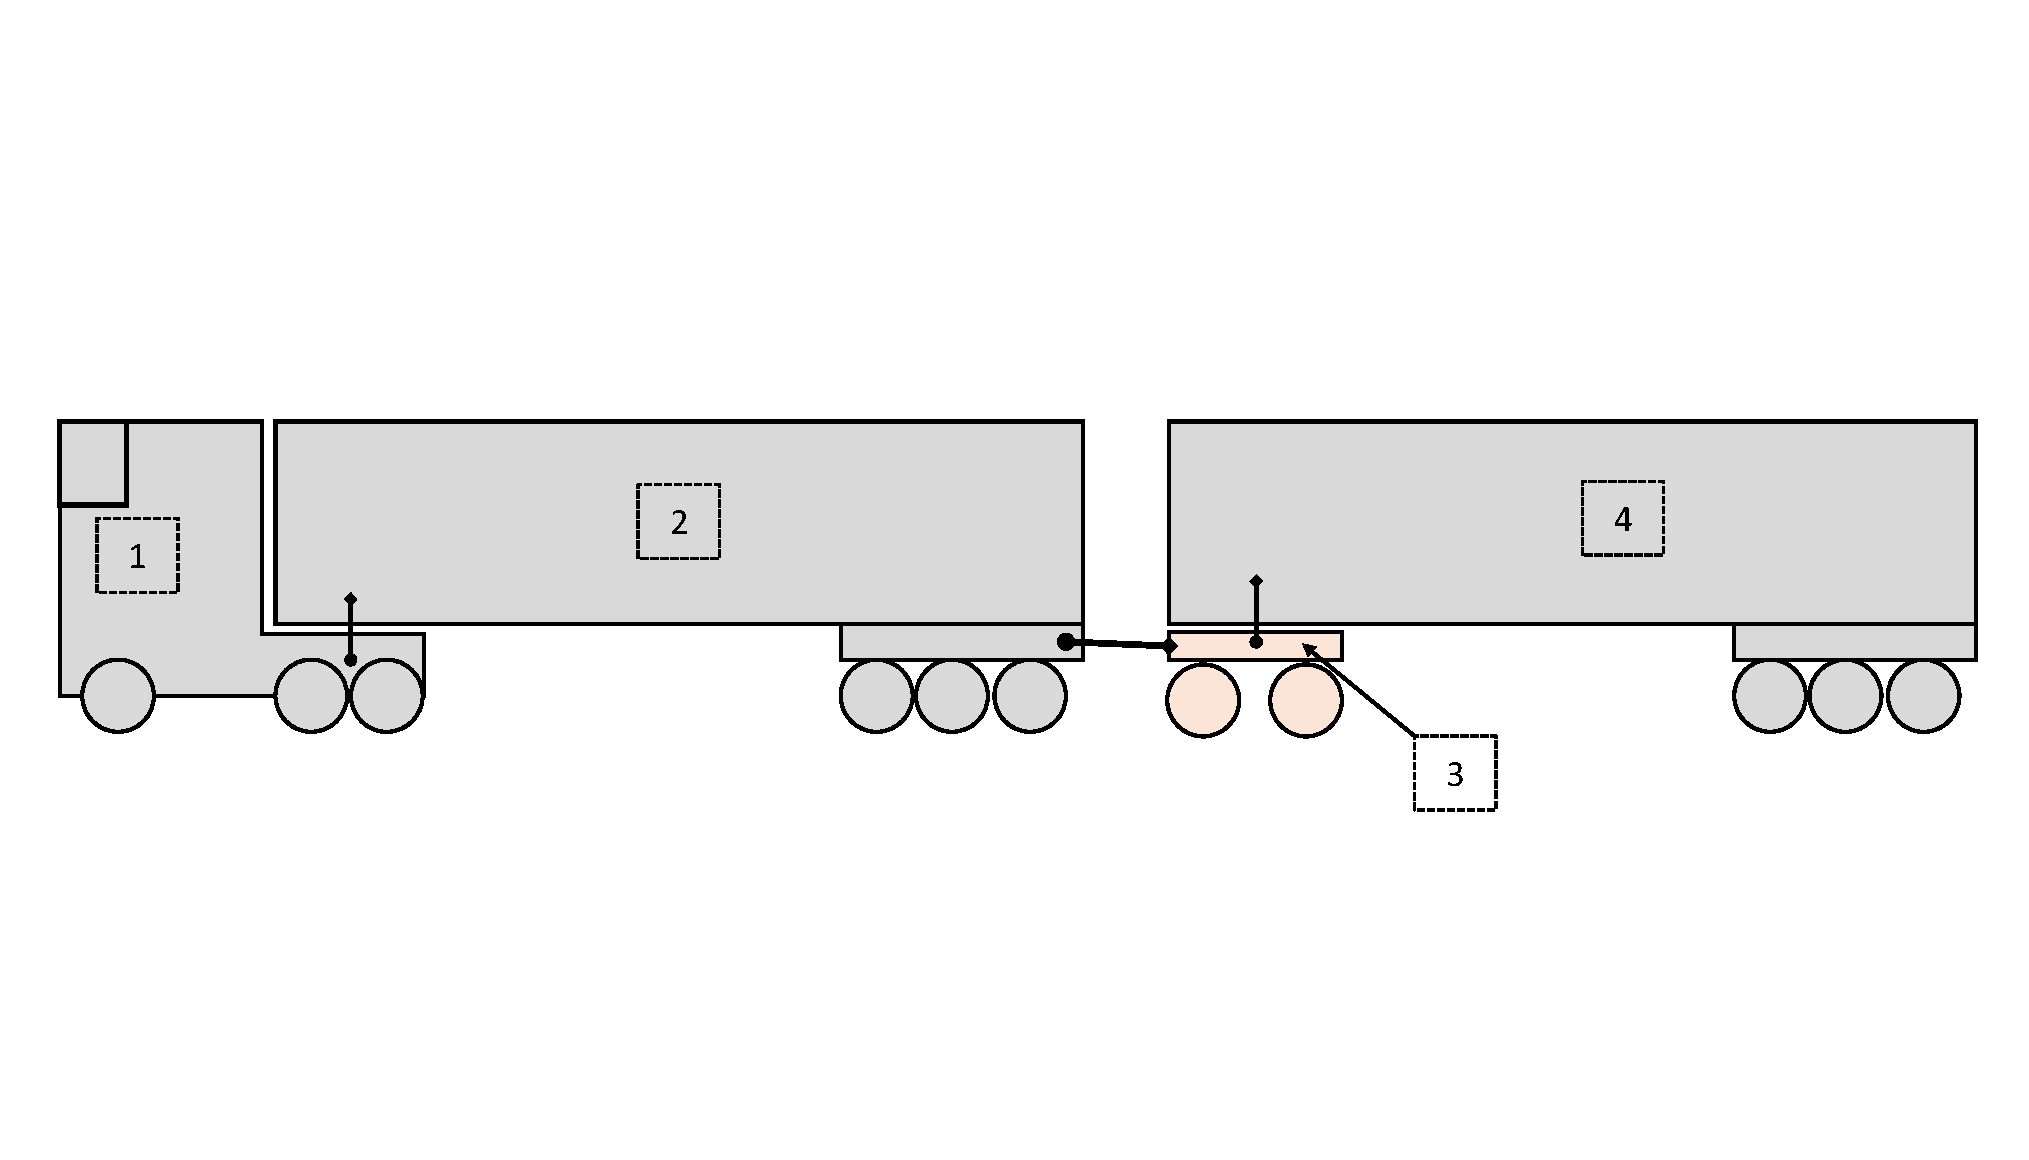
\includegraphics[width=1\linewidth]{figures/combination_overview_with_positions}
\caption{Positioning of different sensors on the LVC}
\label{fig:combination_overview_with_positions}
\end{figure*}

\section{Utilized dolly system}
\label{sec:dolly_system}
The utilized dolly by Parator Industri AB (Parator) is equipped with two steerable axles. They are controlled by an after-market solution called ETS Electronic Trailer Steering System (ETS) supplied by V.S.E. Vehicle Systems Engineering B.V. (VSE), of which figure \ref{fig:legacy_system_vse} gives an overview. Their product includes sensors, ECUs and hydraulic systems which come in a ready-to-mount housing, which is placed on the trailer/dolly. This solution is usually sold as a low-speed active steering system for truck-trailer combinations to provide better maneuverability at low speeds in inner-city areas. Besides electrical power and compressed-air (see "2" in the figure) supply there is no connection with the truck in place. This allows for use with many different truck/trailer original equipment manufacturers (OEM), as no insight into proprietary Controler Area Network communication (CAN) is needed. In the original VSE system the two parameters that influence the actuation of the dolly's steering are vehicle speed ("4") and kingpin-deflection ("3"). This deflection is the angle between the truck and trailer, which is measured by an additional kingpin-angle sensor supplied by VSE and mounted in the eye of the kingpin hub. Furthermore every steering-knuckle of the dolly is equipped with an angle sensor to provide appropriate wheel-individual feedback for the VSE control-system. A diagnosis screen is available in the VSE-unit, which allows for relatively simple set-up, calibration and parametrization to be done.\cite{dolly_datasheet}

VSE provides assisted steering up to a speed of 25km/h over which intervention until it reaches zero at 55km/h. At this treshhold the steerable axles are locked and thus behave like normal rigid axles. This according to the manufacturer is to ensure stability at higher speeds.\cite{dolly_datasheet} Locking the steering at higher speeds leads to a more predictable behaviour for the user and system robustness. However, performance during high speed maneuvers can be improved by uniformly steering the dolly as well.\cite{performance_improvement} The desired demonstration of the algorithm presented in chapter \ref{chap:steering_model} will as outlined in the introduction to this thesis, include steering at higher speeds, thus a work-around had to be established.

\begin{figure}[h]
\centering
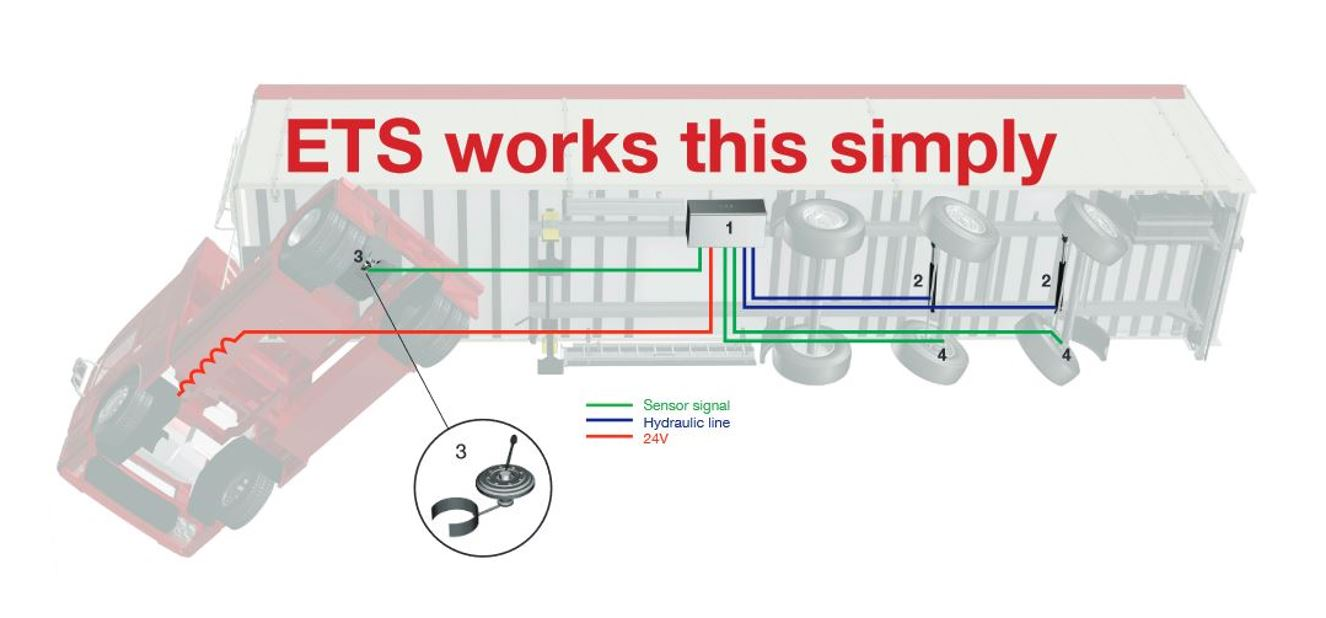
\includegraphics[width=1.0\linewidth]{figures/legacy_system_vse}
\caption[]{Active dolly legacy steering system supplied by VSE\cite{dolly_datasheet}}
\label{fig:legacy_system_vse}
\end{figure}

\begin{figure*}[ph]
\centering
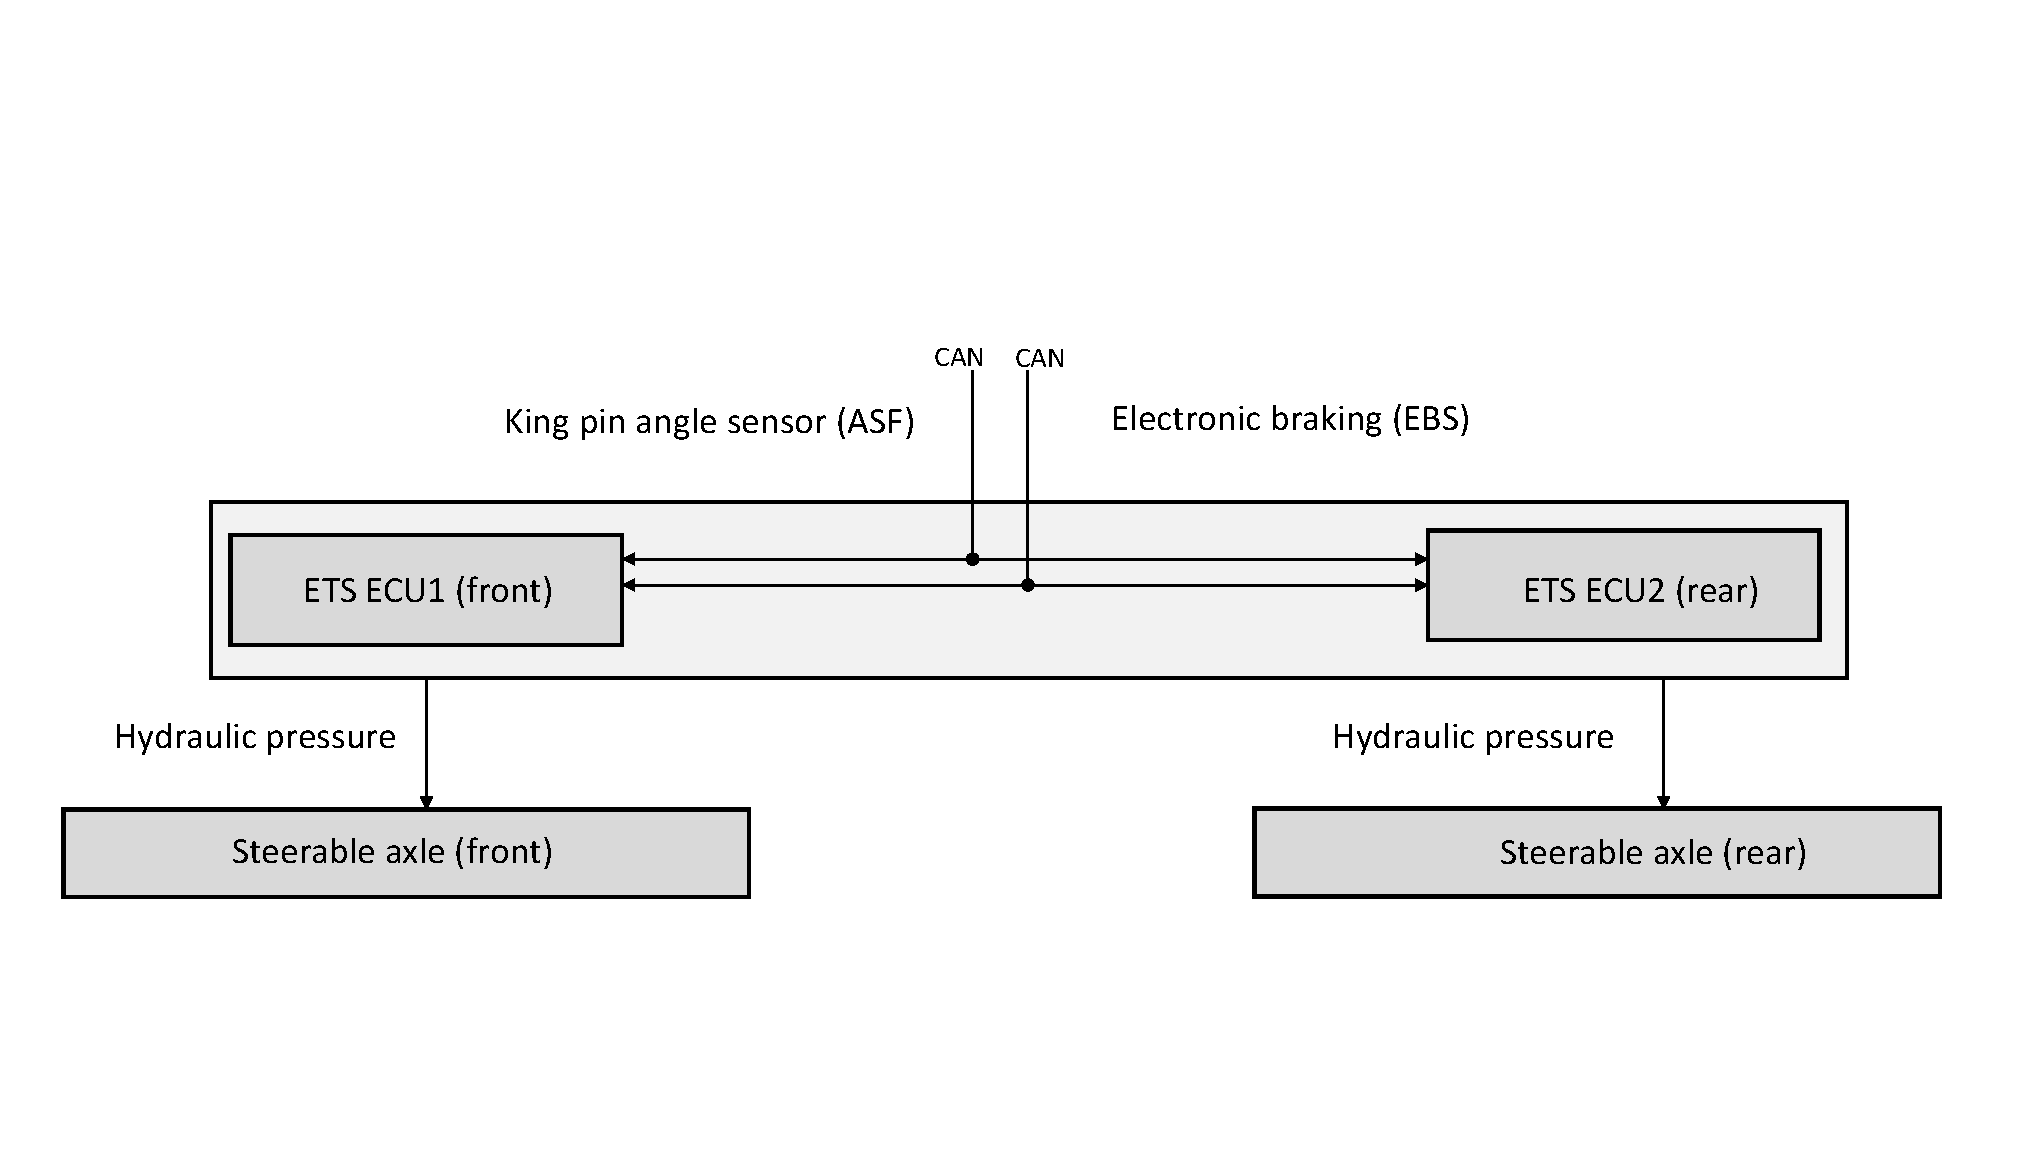
\includegraphics[width=1\linewidth]{figures/system_overview_ETS}

\caption{System overview for sensors and signal path for ETS legacy system by VSE}
\label{fig:system_overview_ETS}
\end{figure*}




Short overview for the dolly, including: 

\begin{itemize}
\item mechanical properties in short (weight, turning radius, max. tonnage)
\item description of function (brake, steer, countersteer, lock at highspeed)
\item difference low $<=>$ high speed
\item control system by VSE, diagnosis, display connection with truck
\item system overview picture/schematics

\end{itemize}
\section{Real-Time Environment}
\label{sec:realtime_environment}



\begin{itemize}
	\item mechanical properties of MABII (dimension, currents, mounting points in dolly)
	\item computational power/limitations
	\item explain interfaces with truck/dolly (abstract)
	\item explain technical realisation of HW interface (ZIF)
	\item explain rapid-prototyping
	\item robustness
	\item programming with software ref to \ref{sec:matlab}
	\item runtime interface ref to \ref{sec:control_desk}
\end{itemize}
\subsection{CAN-bus extension}
\label{sec:can_udp_gateway}
The MABII comes with a preset number of in- and output ports. The maximum number of CAN-buses, that can be connected to the MABII's native controllers is limited to six. As there is no off-the-shelf solution by dSpace for extending the available bus-connections, it was necessary to come up with a gateway solution that allows to patch the needed amount of additional CAN-buses through to the ethernet connection which is also available on the MABII. 

To do so, a gateway from CAN-protocol to the standardized User Datagram protocol (UDP) used for communication on ethernet  infrastructure was implemented. It is a very leight-weight protocol, that is straight-forward to implement and runs well, even with limited processing power on a microcontroller. For future purposes the broadcasting capabilities of UDP might also proof useful, as many nodes could be connected to this CAN-to-UDP gateway for example for visualization on different computers or additional logging outside of the MABII environment. One limitation that was decided on, is to have receiving capabilities only for the MABII to eliminate the need for extensive computation and CAN-matrix handling on the Arduino. \\


\textit{Excursus: The CAN-protocol is the most widespread protocol to allow for communication between different ECUs in the automotive field. Development began at the Robert Bosch GmbH, but is now standardized and enhanced and adjusted for special purposes internationally. Messages are broadcasted by the bus-participants and stamped with their unique identifier, which also doubles as an arbitration token to handle message prioritization. Each bus-participant can listen to all available messages and "only picks from the bus what he needs". The standard message has a size of eight byte \`{a} eight bit, transmitted after the identifier and followed by an ending sequence. Hardware-wise CAN-communication relies on only a pair of twisted wires, where a very robust voltage difference signal is transmitted. }\cite{CAN_intro}\\


By utilizing the UDP-protocol to acquire data into the simulation, the MABII environment's very convenient possibilty to incorporate CAN database files (.dbc-file)\footnote{Correlates physical human readable/understable signals with units to the actual distribution over the different bytes of a CAN-frame. It allows to "decrypt" the information which is available on a CAN-bus and allows to code and send messages in the respective format that the other bus-participants (ECUs, sensors) expect.}, which is the usual way to exchange information and instructions for CAN-networks is no longer available. To decompose the UDP packets into the original signals it was necessary to implement the function of a .dbc-file in the underlying Simulink-model. 

All messages that the CAN-gateway is supposed to handle and forward are put into one UDP frame in succession with respective CAN-identifiers and additional spacer bytes between signals. The UDP frame is broadcasted every time a new CAN-message reaches the gateway on one of its CAN-buses. Messages that were not updated with the incoming CAN-message will be kept at their previous value. This is called for, as UDP is a connection-less protocol without any loss-prevention mechanisms like acknowledgment-handling or retransmission of messages. Holding the values if not available ensures, that at least some value is available on the bus. UDP also doesn't have native 





\begin{figure*}[h]
\centering
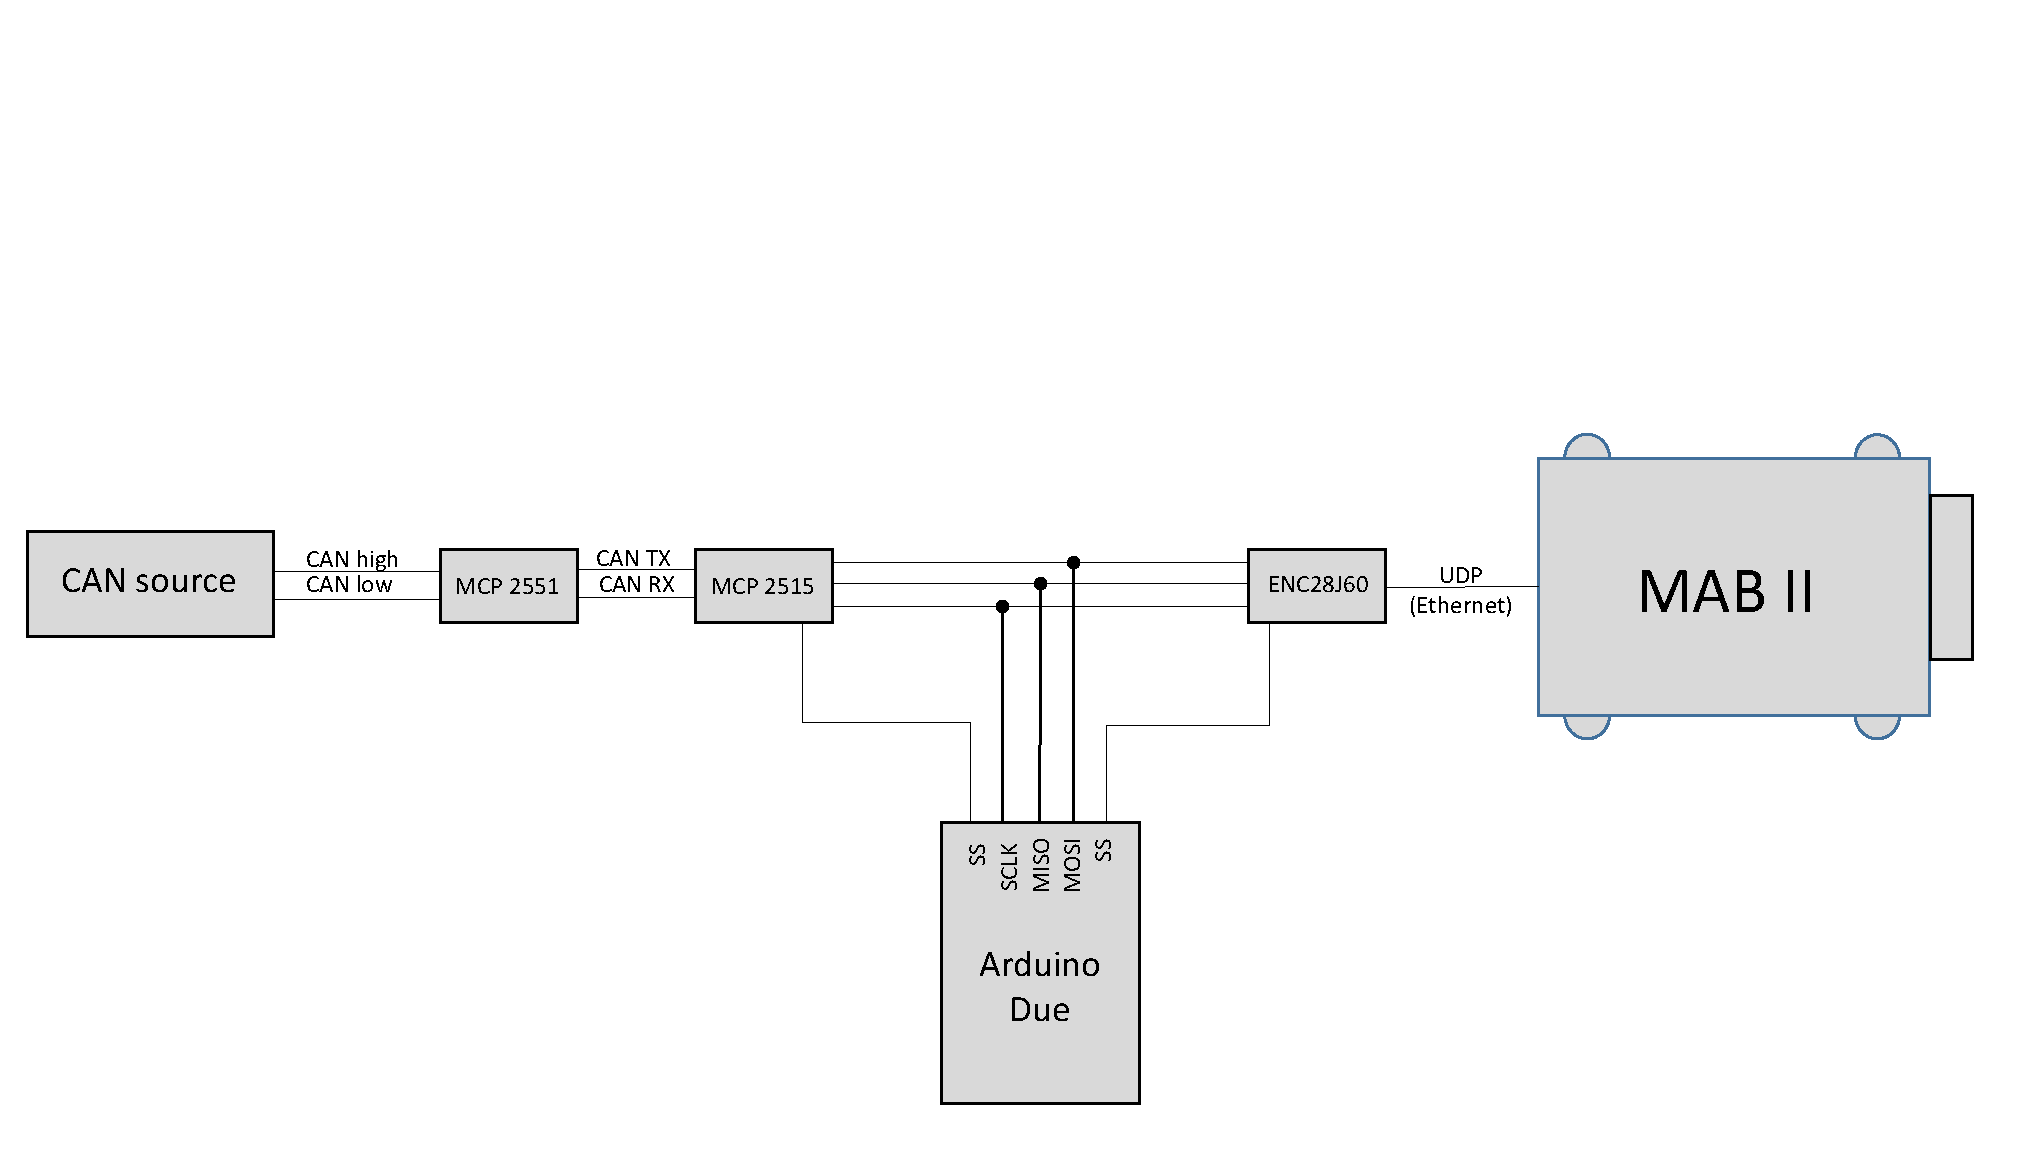
\includegraphics[width=1\linewidth]{figures/can_extension}
\caption{Extension of MABII CAN-buses (hardware overview)}
\label{fig:can_extension}
\end{figure*}


\begin{itemize}
	\item Skalierbarkeit
	\item daten-konvertierung und packaging zu UDP und von UDP zu Daten in CD!!
	\item Skizze des Systems
	\item verwendete bibliotheken
	\item verwendete Controller
	\item I2C-anbindung und bus-layout
\end{itemize}

\section{Interfaces and connections with dolly}
\label{sec:interface_with_dolly}
To control and measure signals of the dolly a connection to the dollies ETS- and EBS-system had to be established. To achieve this, different kinds of CAN-buses had to be used. That was necessary because the various systems of the dolly use different CAN-protocols. In total five CAN-buses connect the MABII with the dolly. Two for each of the ETS-ECUs and one for the ASF- and EBS-Signal.


One of the CAN-buses contains the signals from the EBS-ECUs and the articulation angle sensor, which measures the angle between the dolly and the first semitrailer. It uses the extended CAN-standard. In the original state this CAN is directly routed to the CAN of the two ETS-ECUs (see section \ref{sec:dolly_system}). In order to achieve steering that is both independently from the articulation angle as well as the velocity of the vehicle the connection between the ASF/EBS-CAN and the CAN of the ETS-ECU was cut. Instead the ASF/EBS-CAN is connected to the MABII. \\
The MABII is connected to the CAN bus of each ETS-ECU. Because of the use of different CAN standards of the ASF/EBS-CAN and the ETS-ECU CAN two physical CAN ports are needed on the MABII for each ETS-ECU. Those two CANs are merged inside the breakout-box.
\begin{figure*}[h]
	\centering
	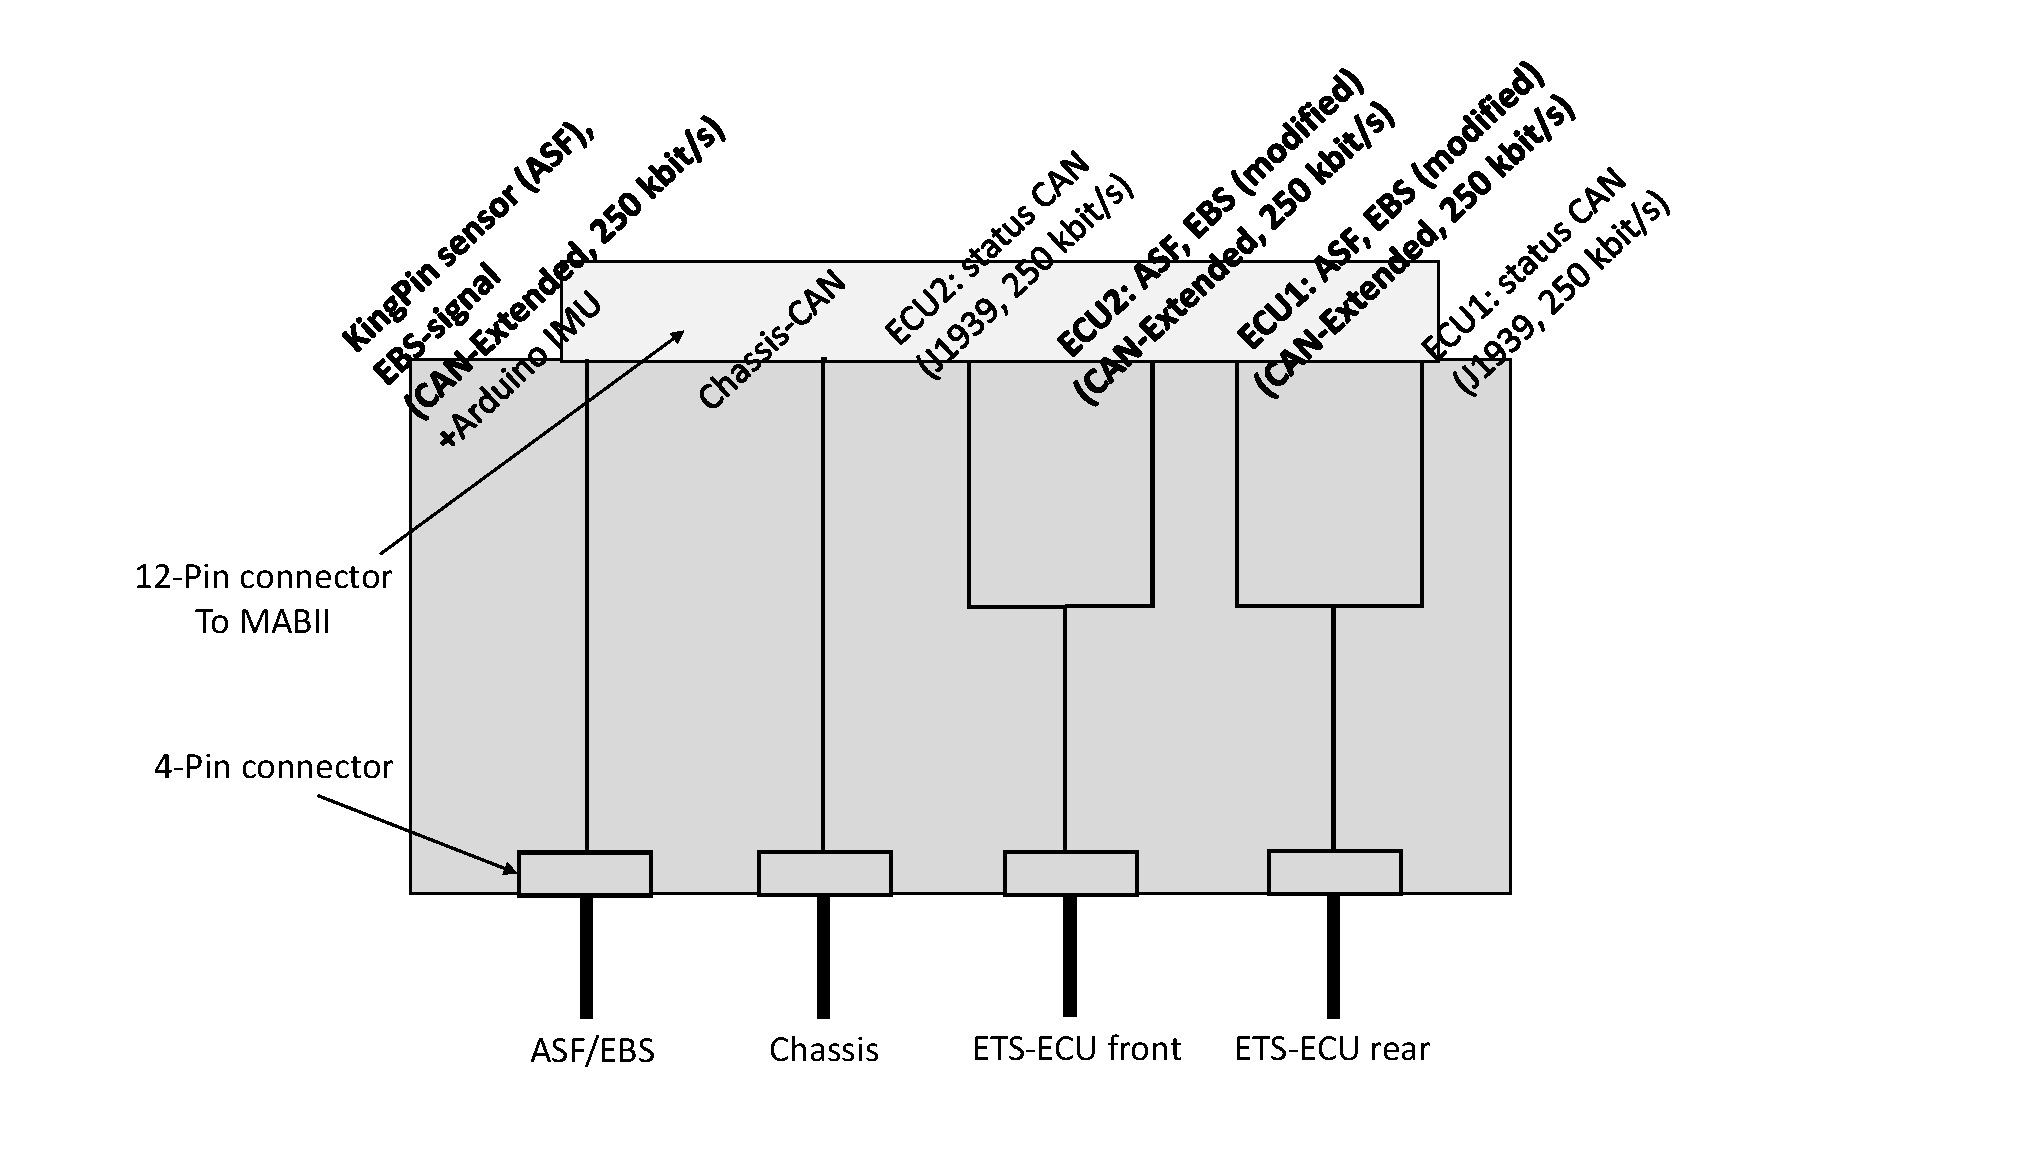
\includegraphics[width=1\linewidth]{figures/BOB_schema}
	\caption{Breakout box scheme}
	\label{fig:BOB}
\end{figure*}
\begin{itemize}
	\item private CANbus with AngleSensor for kingpin\\
	\item Vehicle CAN (ISO 11992, connector ISO 7638-2) \\
	Furthermore there is the ISO 11992 CAN bus which is used for communication between tractor and the attached semitrailers. In the current design this CAN bus isn't connected with the MABII, but for future projects it can be used to control breaking as well as leveling of the dolly.
	\subitem brake by-wire
	\subitem EBS, ABS
	\subitem sensors for EBS, ABS
	\subitem signals/msgs on vehCAN
	\item physial interface =$>$ diagnosis outlet
	\item \textbf{distinguish between HIL/bench-testing and track-testing!!}
\end{itemize}

\section{Interfaces with truck}
\label{sec:interface_with_truck}

\begin{itemize}
	\item CAN communication with truck
	\item steering system conncetion (VDS!)
	\item physical CAN path to dolly?

\end{itemize}


\section{Measurment Setup}
\label{sec:measurement_setup}

\subsection{On-board sensors}

\begin{table}[h]
	\begin{tabular}{llll}
		\textbf{Sensor}       & \textbf{Measurings}                                                 & \textbf{Type} & \textbf{Mounting point} \\
		Draw bar sensor  & \begin{tabular}[c]{@{}l@{}}Kingpin angle\\ Temperature\end{tabular} & External      & TBD!!!                  \\
		EBS                   & wheel speed                                                         & External      & wheel brakes            \\
		Steering angle sensor & steering angle (first, second axle)                                 & External      & steering knuckles      
	\end{tabular}
	\caption{Available sensors of VSE's ETS}
	\label{tab:ets_sensors}
\end{table}





\subsection{Inertial measurement unit}
\label{sec:IMU}
To determine the processing delays in the control chain (refer to chapter \ref{chap:processing_time_delay}) as well as logging implementation for verification and analyses purposes a number of inertial measurement units (IMU) where utilizied throughout this thesis' work. The system at hand combined a gyroscope (L3GD20H), and an accelero- and magnetometer (LSM303D) into an IMU put on one circuit board.\cite{IMU_homepage_shop} This one-chip solution allowed for a convenient access to the sensor measurings, as the sensor outputs could be received via Inter-Integrated Circuit-protocol (I$^{2}$C)  which eliminates the need for a transducer. Furthermore a high-pass filter is integrated into the IMU's accelerometer, which leads to simpler compensation of the immanent drift of the magnetormeter. These units supply the measurings for three axes each at a maximum frequency of 1600Hz for the accelerometer and 757.6Hz for the gyroscope.  \cite{accelerometer_datasheet}\cite{gyrometer_datasheet}

The IMU-chip was put in a suitable plastic housing and cast into resin, to fixate the IMU securily and prevent movement relative to the truck-frame on which it will is mounted as well as ensuring water-proofing.

Figure \ref{fig:IMU_overview} shows, how the IMU is connected to the Arduino Due utilizing the I$^{2}$C-interface on the Due. Not pictured are the power supplies (both 5V) for the MCP2515 CAN-transceiver and the IMU itself. To minimize cables that have to be rooted through the combination and avoid problems with cable length for the power cables, it was decided to equip each of these assemblies with a rechargeable battery-pack. This also allows to measure in remote location and collect data locally on the Arduino Due during testing, eliminating the need for CAN-communication completely if needed in the future.

A maximum of two IMUs can run on one I$^{2}$C line as it is possible to override the last bit of the otherwise hard-coded I$^{2}$C address via a hardware jumper. If both I$^{2}$C lines of the Due are used, it would be possible to connect up to four IMUs to one Arduino. Though eight IMUs are desired for the whole LCV, this was outruled as a possibility for this project, due to the limitations of the physical bus-length of the I$^{2}$C lines of only a few meters (as the name already suggests I$^{2}$C is not meant for long distance communication). As can also be seen in the overview figure of the setup on the truck in figure \ref{fig:combination_overview_with_positions} this distance would be exceeded with the distance between the different mounting points (15-20m).

In the final measuring setup the assembly shown in figure \ref{fig:IMU_overview} will be present four times in the whole combination, to gather motion data from each independently moving part. Figure \ref{fig:combination_overview_with_positions} shows those placements in an overview sketch. The correct placement will be as close as possible to the center of gravity (CoG) of the respective unit to have as little influence of the vehicle's rotary motions as possible, which drastically reduces work in  data analysis further on. CoG locations can be gathered from Volvo's internal database and are available at the test site. Putting two IMUs in each spot allows for averaging and ensure redundancy should one IMU chip fail or produce corrupt outputs, which occured from time to time during the bench-testing of the assembly if the voltage of the preliminary power-supply dropped due to other loads.

\begin{figure*}[h]
\centering
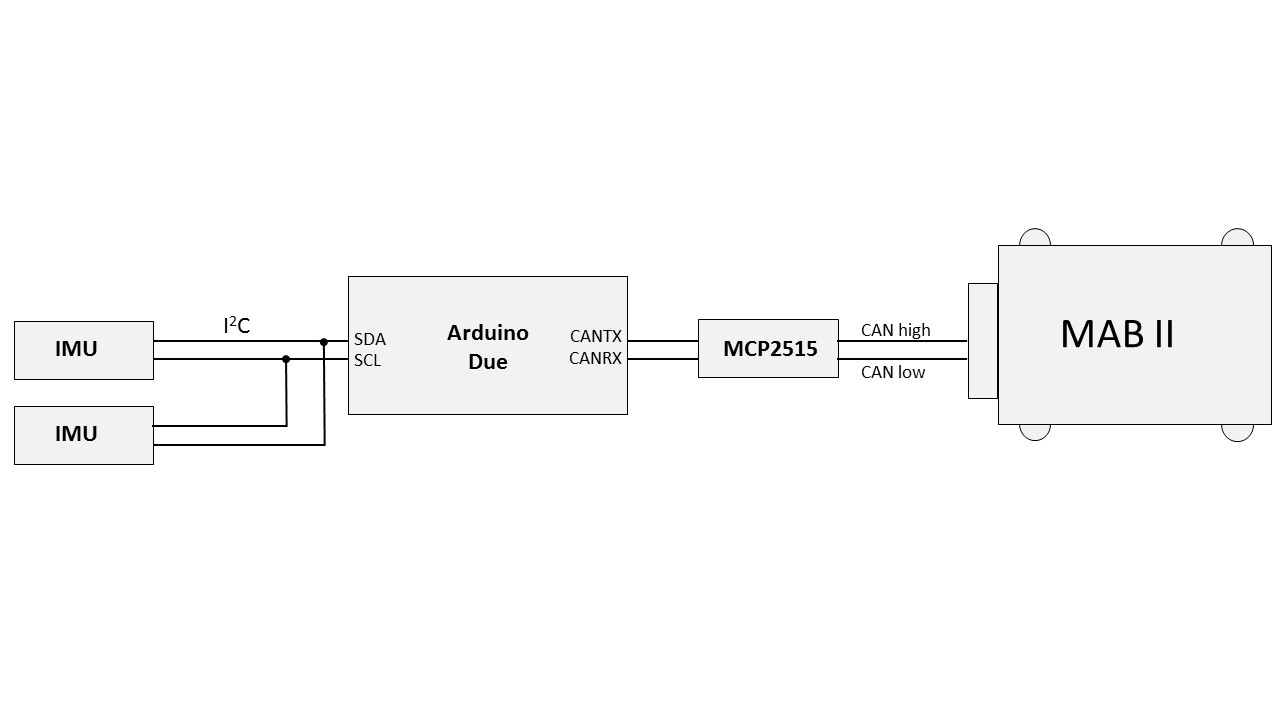
\includegraphics[width=1\linewidth]{figures/IMU_overview}
\caption{Connection of IMU with Arudino Due to MABII}

\label{fig:IMU_overview}
\end{figure*}



\subsection{Arduino Due}
\label{sec:arduino}

To parse the IMU's sensor output (see also section \ref{sec:IMU}) and convert it into a measurable format and for the implementation of the CAN-to-UDP gateway, it was decided to rely on the cost-efficient and flexible Arduino microcontroller platform. The Arduino platform series was developed by  SmartProjects company in Italy and consists of a micro-controller board with several in- and output pins, and a set of programming tools to program said micro-controller (see also section \ref{sec:arduino_applications}). Hardware layouts as well as software of this solution are released under an open-source licence, so changes at any level of detail can be made and many other suppliers are now offering solution that tie in with the Arduino. Furthermore this lead to a broad user base and availability of vast supporting resources.

SmartProjects offers various Arduino boards mainly differing in number of communication pins, memory size, clock frequency and physical size. It was decided to utilize the to date most powerful Arduino Due, offering 84 MHz of clock-speed on a ARM Cortex-M3 processor, 512kB flash memory for programm-code and a 96kB working SRAM. It is the first Arduino with 32-bit architecture. This was done in order to allow for future use of this platform in other projects and having enough space for different sub-programs on the controller as well as enough processing power to deal with basic signal filtering and parsing at appropriate speeds. 

The Due has a native I$^{2}$C interface, which was used to gather the measurings from the IMU. It also has a Serial Peripheral Interface interface (SPI) which is needed to access the ethernet controller necessary for the CAN-UDP-gateway (refer to section \ref{sec:can_udp_gateway}), serial communication is also handled on hardware level. The availability of these ports in hardware form allow for robust systems and eliminate the need to implement those protocols on software level (bit-banging), which frees up memory resources. In addition to this digital communication possibilities the Due offers an abundance of 54 digital and 12 analog freely configurable I/O-pins. The Due is also the first Arduino to host an on-board CAN-controller, which in this thesis will be used for measurement transfer to the logging system (MABII), eliminating the need for additional hardware for CAN-bus interfacing on the Arduino side.

Besides the power-supply and the IMU-chip a MCP2551 CAN-transceiver by Microchip Technology Inc. was incorporated to take care of the pyhsical layer of CAN-bus communication by converting the digital signals from the Due's CAN-controller to the standardized voltage levels of the CAN. The MCP2551 is capable of different CAN standards and fully ISO-11898 compatible, which makes future use in different environments or as unit for in-vehicle CAN-interfacing feasible.

The Arduino Due was used to determine the delays in the system (see section \ref{sec:measuring_delay}) as well as a light-weight solution to quickly read CAN-outputs of the various systems during this thesis' work. This proofed to be an easy debugging solution. Additionally it was used to trigger some error codes to test the developed safety mechanisms (see section \ref{sec:fault_detect_test}). 

%\begin{itemize}
	%\item clock frequency
	%\item RAM/ROM
	%\item ISP flash
	%\item robustness, reliability, cost-effectiveness
	%\item input/outputs analog $\&$ digital
	%\item native I2C capability
	%\item CANcomm except of physical layer/transceiver available (OSI reference!) --$>$ no bit-banging needed --$>$ faster
%\end{itemize}





\end{document}
